\documentclass[conference]{IEEEtran}
\IEEEoverridecommandlockouts

\usepackage{cite}
\usepackage{amsmath,amssymb,amsfonts}
\usepackage{algorithmic}
\usepackage{graphicx}
\usepackage{textcomp}
\usepackage{xcolor}
% Added for the generated result tables and links.
\usepackage{iftex}
\ifXeTeX
  % XeTeX/Tectonic builds lack the Type-1 Times that IEEEtran uses under pdfLaTeX.
  \usepackage{fontspec}
  \setmainfont{texgyretermes}[Extension=.otf, UprightFont=*-regular, BoldFont=*-bold,
    ItalicFont=*-italic, BoldItalicFont=*-bolditalic]
\fi
\usepackage{booktabs}
\usepackage{array}
\usepackage{url}
\usepackage{tikz}
\usetikzlibrary{positioning,arrows.meta,fit,calc}
\usepackage[hidelinks]{hyperref}

\def\BibTeX{{\rm B\kern-.05em{\sc i\kern-.025em b}\kern-.08em
T\kern-.1667em\lower.7ex\hbox{E}\kern-.125emX}}

% Visible placeholder for anything the team still has to check or decide.
% The submitted version must compile with zero \todo occurrences.
\newcommand{\todo}[1]{\textcolor{red}{[TODO: #1]}}

\begin{document}

% ============================================================
% TITLE
% ============================================================

\title{
Residual TFT-EWC: Continual Learning for State-of-Health Forecasting
and Reuse Screening of Heterogeneous Second-Life EV Batteries
}

% ============================================================
% AUTHORS
% ============================================================

\author{
\IEEEauthorblockN{Tarun Sitaraman}
\IEEEauthorblockA{
\textit{Department of Networking and}\\
\textit{Communications}\\
\textit{SRM Institute of Science}\\
\textit{and Technology}\\
Chennai, India
}
\and
\IEEEauthorblockN{Sohan Sandeep Krishnan}
\IEEEauthorblockA{
\textit{Department of Networking and}\\
\textit{Communications}\\
\textit{SRM Institute of Science}\\
\textit{and Technology}\\
Chennai, India
}
\and
\IEEEauthorblockN{Darshan D}
\IEEEauthorblockA{
\textit{Department of Networking and}\\
\textit{Communications}\\
\textit{SRM Institute of Science}\\
\textit{and Technology}\\
Chennai, India
}
}

\maketitle

% ============================================================
% ABSTRACT
% ============================================================

\begin{abstract}
Retired electric-vehicle batteries can be reused in less demanding applications, but a health model trained on one battery population may fail on the next. Continual learning addresses this by adapting to each new population without forgetting earlier ones. We propose Residual TFT-EWC, a Temporal Fusion Transformer with Elastic Weight Consolidation that learns a shrunk correction to linear extrapolation, and use it to forecast the state of health (SOH) of lithium-ion cells one to six capacity checks ahead. On a leakage-controlled benchmark from five public datasets (395 cells), with pre-registered experiments and every claimed difference replicated on a second seed set, it is compared with fine-tuning, replay, joint training, literature backbones and simple forecasters. Forgetting appears whenever usage conditions differ (up to 0.46 percentage points, pp). Of the models compared, Residual TFT-EWC is the only one that stays competitive both on a continual stream and on unseen usage conditions. On the stream, it matches the strongest baseline, linear extrapolation, and is 0.13--0.41~pp more accurate than gradient boosting, and EWC cuts its forgetting at longer horizons by about two thirds. On unseen conditions, where extrapolation degrades, it is 0.43--0.68~pp more accurate than extrapolation and assigns the measured capacity-based health class to 95.5\% of samples. Gradient boosting and the jointly trained TFT are more accurate there mainly because they store every earlier condition's data; held to the same no-storage constraint, gradient boosting is within 0.08~pp of our model. Forecast intervals reach nominal coverage on a new condition when calibrated on conditions held out from fitting, except outside the training range.
\end{abstract}

% ============================================================
% KEYWORDS
% ============================================================

\begin{IEEEkeywords}
Continual learning, second-life batteries, electric vehicles, state of health, battery degradation, heterogeneous batteries, catastrophic forgetting, machine learning
\end{IEEEkeywords}

% ============================================================
% I. INTRODUCTION  (team draft, condensed to the IEEE conference length)
% ============================================================

\section{Introduction}

When an electric-vehicle (EV) battery can no longer meet the demands of driving, it can often still serve as stationary storage or backup power. Reusing it extends its life and delays recycling, but only if its health can be judged reliably.

The state of health (SOH) compares a battery's present capability with a reference state. Machine-learning models have estimated it from voltage, current, temperature, partial-charging and impedance measurements~\cite{ref1,ref2,ref3,ref4}. Retired batteries, however, differ in chemistry, maker, capacity, past use, temperature and charging, and their records from first use are often incomplete, so a model trained once may fail on the next group. Continual learning updates a model with each new group while trying to keep what it learned before.

This work brings together continual learning, health forecasting and a first screening step for reuse. Rather than estimate today's SOH, we \emph{forecast} it one to six capacity checks ahead from everything measured up to the latest check. On our first dataset, estimating the current SOH from cycling data did worse than simply repeating the last measured value (\S\ref{sec:methods}), and a reuse decision depends on how a battery will age, not only on its health today. The forecast is then sorted into capacity-based classes that support, but do not replace, a full reuse assessment.

% System architecture of the study (Fig. 1). Drawn in TikZ; every number is from Section III.
\begin{figure*}[t]
  \centering
  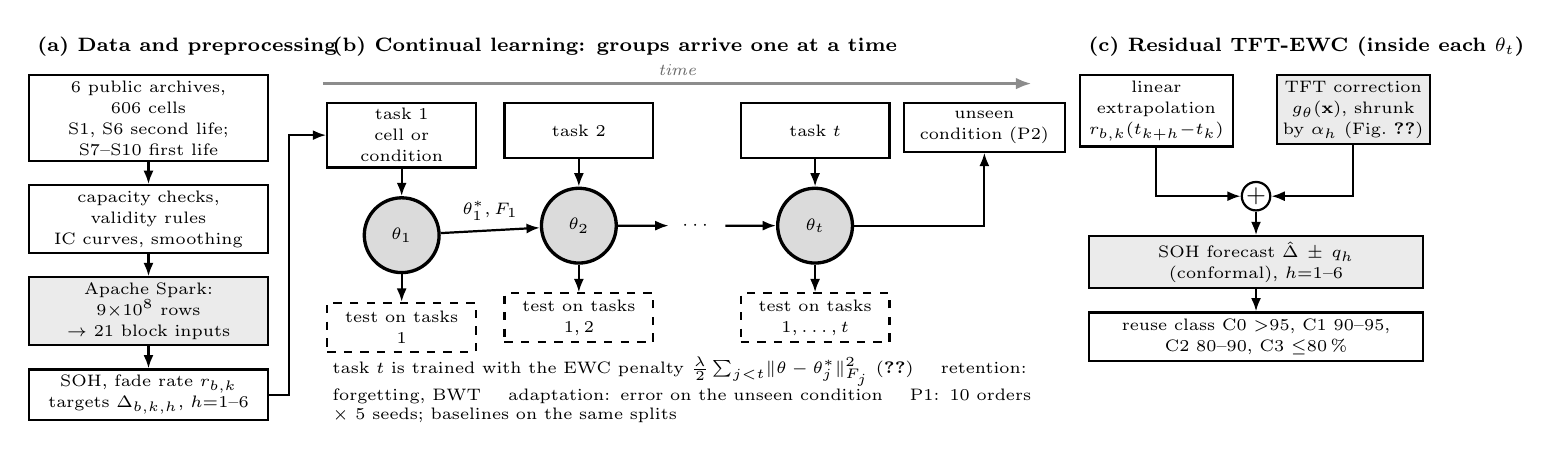
\begin{tikzpicture}[
      font=\fontsize{6.4}{7.6}\selectfont,
      box/.style={draw, thick, rectangle, align=center, inner sep=2pt, minimum height=0.62cm},
      key/.style={box, fill=black!8},
      hero/.style={box, very thick, fill=black!14},
      flow/.style={-{Latex[length=1.7mm]}, thick},
      tier/.style={font=\fontsize{6.8}{7.8}\selectfont\bfseries, align=center}]
    % (a) data and preprocessing
    \node[tier, anchor=west] at (0,0.35) {(a) Data and preprocessing};
    \node[box, text width=2.9cm, anchor=north west] (a1) at (0,0) {6 public archives, 606 cells\\S1, S6 second life; S7--S10 first life};
    \node[box, text width=2.9cm, below=0.28cm of a1] (a2) {capacity checks, validity rules\\IC curves, smoothing};
    \node[key, text width=2.9cm, below=0.28cm of a2] (a3) {Apache Spark: $9{\times}10^{8}$ rows\\$\rightarrow$ 21 block inputs};
    \node[box, text width=2.9cm, below=0.28cm of a3] (a4) {SOH, fade rate $r_{b,k}$\\targets $\Delta_{b,k,h}$, $h{=}1$--6};
    \foreach \a/\b in {a1/a2,a2/a3,a3/a4} \draw[flow] (\a) -- (\b);

    % (b) continual task stream
    \node[tier, anchor=west] at (3.75,0.35) {(b) Continual learning: groups arrive one at a time};
    \draw[-{Latex[length=2mm]}, black!45, line width=1.2pt] (3.75,-0.12) -- (12.75,-0.12)
      node[pos=0.5, above=-1pt, black!60, font=\fontsize{6}{7}\selectfont\itshape] {time};
    \foreach \i/\x/\t/\m/\e in {1/4.75/{task 1\\cell or condition}/{\theta_1}/{1},
                                2/7.0/{task 2}/{\theta_2}/{1,2},
                                3/10.0/{task $t$}/{\theta_t}/{1,\dots,t}} {
      \node[box, text width=1.75cm, minimum height=0.7cm, anchor=north] (T\i) at (\x,-0.35) {\t};
      \node[hero, circle, minimum size=0.95cm, inner sep=0pt, below=0.35cm of T\i] (M\i) {$\m$};
      \draw[flow] (T\i) -- (M\i);
      \node[box, dashed, text width=1.75cm, below=0.35cm of M\i] (E\i) {test on tasks\\$\e$};
      \draw[flow] (M\i) -- (E\i);
    }
    \node at ($(M2)!0.5!(M3)$) {$\cdots$};
    \draw[flow] (M1) -- node[above, font=\fontsize{6}{7}\selectfont] {$\theta^*_1, F_1$} (M2);
    \draw[flow] (M2) -- ($(M2)!0.38!(M3)$);
    \draw[flow] ($(M2)!0.62!(M3)$) -- (M3);
    \node[box, text width=1.9cm, anchor=north] (U) at (12.15,-0.35) {unseen\\condition (P2)};
    \draw[flow] (M3) -| (U);
    \node[align=left, anchor=north west, text width=8.9cm, font=\fontsize{6}{7}\selectfont] at (3.75,-3.47)
      {task $t$ is trained with the EWC penalty $\tfrac{\lambda}{2}\sum_{j<t}\lVert\theta-\theta^*_j\rVert^2_{F_j}$~\eqref{eq:ewc} \quad
       retention: forgetting, BWT \quad adaptation: error on the unseen condition \quad
       P1: 10 orders $\times$ 5 seeds; baselines on the same splits};

    % (c) the model inside each state
    \node[tier, anchor=west] at (13.35,0.35) {(c) Residual TFT-EWC (inside each $\theta_t$)};
    \node[box, text width=1.8cm, anchor=north west] (lin) at (13.35,0) {linear\\extrapolation\\$r_{b,k}(t_{k+h}{-}t_k)$};
    \node[key, text width=1.8cm, anchor=north west] (tft) at (15.85,0) {TFT correction\\$g_\theta(\mathbf{x})$, shrunk\\by $\alpha_h$ (Fig.~\ref{fig:arch})};
    \node[draw, thick, circle, inner sep=0.3pt, font=\small] (sum) at (15.6,-1.55) {$+$};
    \draw[flow] (lin.south) |- (sum); \draw[flow] (tft.south) |- (sum);
    \node[key, text width=4.1cm, below=0.3cm of sum] (fc) {SOH forecast $\hat\Delta\pm q_h$ (conformal), $h{=}1$--6};
    \node[box, text width=4.1cm, below=0.28cm of fc] (cl) {reuse class C0 $>$95, C1 90--95,\\C2 80--90, C3 $\le$80\,\%};
    \draw[flow] (sum) -- (fc); \draw[flow] (fc) -- (cl);

    \draw[flow] (a4.east) -- ++(0.25,0) |- (T1.west);
  \end{tikzpicture}
  \caption{System architecture. (a) Archives to labels and inputs. (b) Groups arrive as tasks; each state $\theta_t$ is
    trained with EWC and tested on all tasks so far and on unseen conditions. (c) The forecast of each state.}
  \label{fig:system}
\end{figure*}


Fig.~\ref{fig:system} summarises the approach, and the paper makes four contributions. First, we build a benchmark for forecasting the SOH of second-life cells from six public datasets (606 cells after quality checks) so that no future information reaches the inputs, and we remove two label flaws: test currents set from the previous capacity, and pulse charge counted as capacity. Second, we compare a Temporal Fusion Transformer with Elastic Weight Consolidation (TFT\,+\,EWC) with fine-tuning, replay, joint training, simple forecasters and the model types of earlier work when groups arrive in sequence, when groups are unseen and after first-life pretraining, reporting both adaptation and forgetting. Third, we propose Residual TFT-EWC, which corrects linear extrapolation instead of replacing it. Among methods that keep no earlier data, it is the only one close to the best in both settings: it matches extrapolation on the stream, where EWC cuts its forgetting by about two thirds, outperforms it on unseen usage conditions, and beats gradient boosting refitted on each new condition on the stream (replicated). Keeping 40 rows per condition, a post hoc replay variant shows no replicated difference from joint training on two many-condition datasets; gradient boosting with all data stored stays better on one. Finally, we give forecast intervals for unseen conditions, which reach the stated coverage only when calibrated on conditions left out of training and within the training range, and a reproducibility check: because significance on these small datasets changed with the computing platform, our main results must pass a replication rule.


% ============================================================
% II. RELATED WORK  (team draft, condensed to the IEEE conference length)
% Bibliographic data of all ten studies verified against Crossref (4 Oct 2026). Figures quoted for
% ref1, ref2, ref4, ref5, ref8 and ref10 were checked against the published abstracts. For ref3, ref6,
% ref7 and ref9 no open abstract was available, so the text states only what their titles state.
% tao2026pcl (added 2 Nov 2026): described from its abstract only (Chalmers research record).
% ============================================================

\section{Related Work}

We review studies from 2022--2026 (Table~\ref{tab:literature}; a broader review is~\cite{ref6}). Second-life studies estimate the \emph{current} SOH of a fixed set of batteries: from partial charging under residential and fast-charging profiles (RMSE about 0.6 and 0.8\%, with 85\% less testing time than a capacity test)~\cite{ref1}, from 58 health indicators of reused Nissan Leaf modules (about 0.2\% RMSE, though the most useful indicators changed with ageing)~\cite{ref2}, from impedance spectra~\cite{ref3}, with bagged Gaussian process regression for screening (worst-case error below 1.48\%)~\cite{ref4}, and online, with clustering, for Leaf cells aged over 15 months (error below 2.3\%)~\cite{ref5}. None updates its model as new groups arrive.

Continual learning has been used to predict capacity loss~\cite{ref7} and, with progressive networks and TCNs, the state of charge across drive cycles, with attention to forgetting and task order~\cite{ref8}. Closest to our setting, pulse-test conditions have been learned one after another, with a replay buffer, to estimate second-life SOH with almost no forgetting~\cite{tao2026pcl}. Domain generalisation~\cite{ref9} and probabilistic BiLSTM/TCN models with isotonic recalibration~\cite{ref10} also target second-life SOH, but without a sequence of tasks.

\begin{table}[t]
  \centering
  \caption{Approaches of the reviewed studies and of this work. Their errors are not comparable with ours (other
    cells, targets and SOH definitions).}
  \label{tab:literature}
  \scriptsize
  \setlength{\tabcolsep}{2.5pt}
  \begin{tabular}{p{1.05cm}p{2.75cm}p{2.35cm}cc}
    \toprule
    Study & Approach & Predicts & CL & Reuse \\
    \midrule
    \cite{ref1} & partial-charge features & current SOH, second life & -- & -- \\
    \cite{ref2} & 58 health indicators & current SOH, second life & -- & -- \\
    \cite{ref3} & impedance (EIS) + ML & current SOH, second life & -- & -- \\
    \cite{ref4} & statistical features, bagged GPR & current SOH, screening & -- & \checkmark \\
    \cite{ref5} & online ML, clustering & current health, second life & -- & -- \\
    \cite{ref7} & bilevel-optimised CL & capacity degradation & \checkmark & -- \\
    \cite{ref8} & PNN + TCN & state of charge & \checkmark & -- \\
    \cite{tao2026pcl} & pulse features, replay CL & current SOH, second life & \checkmark & -- \\
    \cite{ref9} & domain generalisation & current SOH, second life & -- & -- \\
    \cite{ref10} & BiLSTM, TCN, TCN-GPR & SOH with uncertainty & -- & \checkmark \\
    \midrule
    This work & residual TFT + EWC, shrinkage, conformal intervals & SOH 1--6 checks ahead, interval & \checkmark & \checkmark \\
    \bottomrule
  \end{tabular}
\end{table}

\emph{Research gap.} So far, continual learning for second-life SOH has \emph{estimated} the current SOH~\cite{tao2026pcl}. To our knowledge, it has not been tested for \emph{forecasting} across different groups of second-life batteries, together with reuse screening, a measure of forgetting, and a comparison with simple forecasters and with training on all data at once. We ask whether a continual learner can learn such groups one after another without losing the earlier ones, and whether its forecasts support reuse screening.

% =============================================================================
% Methodology (condensed to the IEEE conference length)
%
% Written from the implementation and docs/DECISIONS.md (D11, D12, D14, D16-D21).
% Data sources: docs/EXTERNAL_DATA.md. Every number in this section is traceable
% to results/*.json on a clean commit or to the data report (docs/DATA_REPORT.md).
% The full protocol, feature lists and data-quality rules are in the repository.
% =============================================================================

\section{The Residual TFT-EWC Approach}
\label{sec:methods}

We forecast the SOH one to three checks ahead (up to six in later experiments) from everything measured up to a reference performance test (RPT), i.e.\ a capacity check, with cells or usage conditions arriving as tasks. Estimating the \emph{current} SOH failed on the first dataset: cycle-level features carried almost no health information (median within-cell Spearman correlation with SOH 0.09, against $-0.99$ for elapsed time), and gradient boosting and ridge (1.78, 2.37~pp) lost to persistence, which repeats the last measured SOH (0.99~pp). We therefore switched to forecasting after seeing the data, fixing the protocol before fitting any forecaster.

% -----------------------------------------------------------------------------
\subsection{Datasets}
\label{sec:data}

Table~\ref{tab:data} lists the six public datasets (all CC~BY~4.0). Every file is checked against its repository record or checksums, and our parsing of the raw files exactly reproduces the processed S1 RPT capacities and the authors' capacities of all 843 S6 checks.

\begin{table}[t]
  \centering
  \caption{Datasets. S1 and S6 form the continual-learning streams; S7--S9 form the first-life pretraining pool; S7 and S10 give the many-condition tests.}
  \label{tab:data}
  \scriptsize
  \setlength{\tabcolsep}{2.5pt}
  \begin{tabular}{p{0.95cm}p{3.0cm}p{1.75cm}r}
    \toprule
    Set & Cells and conditions & Label & Samples \\
    \midrule
    S1~\cite{moy2024secondlife,moy2024secondlifedata} & 6 NMC 21700 cells, second life on residential or commercial peak shaving, 20/35~$^\circ$C blocks & C/20 RPT capacity, pulses excluded & 279 \\
    S6~\cite{wheeler2025lfp,wheeler2025lfpdata} & 20 LFP 18650 cells, 7 conditions (charge mode, voltage and rate, discharge, depth), 50~$^\circ$C & C/25 check capacity & 2{,}409 \\
    S7~\cite{luh2024agingdata,luh2024agingdatav2} & 195 of 228 NMC/C+SiO cells, calendar, cyclic and WLTP ageing, 0--40~$^\circ$C & check-up capacity & 10{,}251 \\
    S8~\cite{wang2024pinn,wang2024pinndata} & 55 NCM cells, six charge/discharge protocols & capacity cycles & 9{,}699 \\
    S9~\cite{zhu2022relaxation,zhu2022relaxationdata} & 119 of 130 NCA, NCM and blended cells, 25--45~$^\circ$C & capacity cycles & 16{,}761 \\
    S10~\cite{stroebl2024agingdata,stroebl2024agingdatafig} & 211 of 279 NMC 21700 cells, 71 calendar and cyclic conditions, 10--45~$^\circ$C & check-up capacity & 6{,}495 \\
    \bottomrule
  \end{tabular}
\end{table}

\emph{S1} contains six LG~Chem INR21700-M50T cells that spent 23 months under an EV driving profile~\cite{pozzato2022firstlife} and then about 27 months on peak-shaving duty cycles~\cite{moy2023dutycycles}; each RPT is a C/20 discharge interrupted by C/2 pulses, with impedance spectroscopy (EIS) from the fifth RPT~\cite{moy2024secondlife}. RPT~2, run at about 20~$^\circ$C, is dropped.

\emph{S6} was chosen by criteria fixed before the search (licence, a series of capacity checks, ageing past the end of first life, and the variety that S1 lacks). Its cells were checked every 100 cycles and end at 32--64\% SOH; here ``second life'' means further ageing below 80\% SOH under the same test. A check is used only if its C/25 discharge starts from full charge and reaches the cut-off voltage (843 of 847; Fig.~\ref{fig:prep}). From the first-life sets \emph{S7--S9} we keep cells with at least five valid checks (369 cells, 36{,}711 samples). \emph{S10} uses the discharge capacity of each 23~$^\circ$C check-up (2{,}587 of 2{,}766 kept).

\begin{figure*}[t]
  \centering
  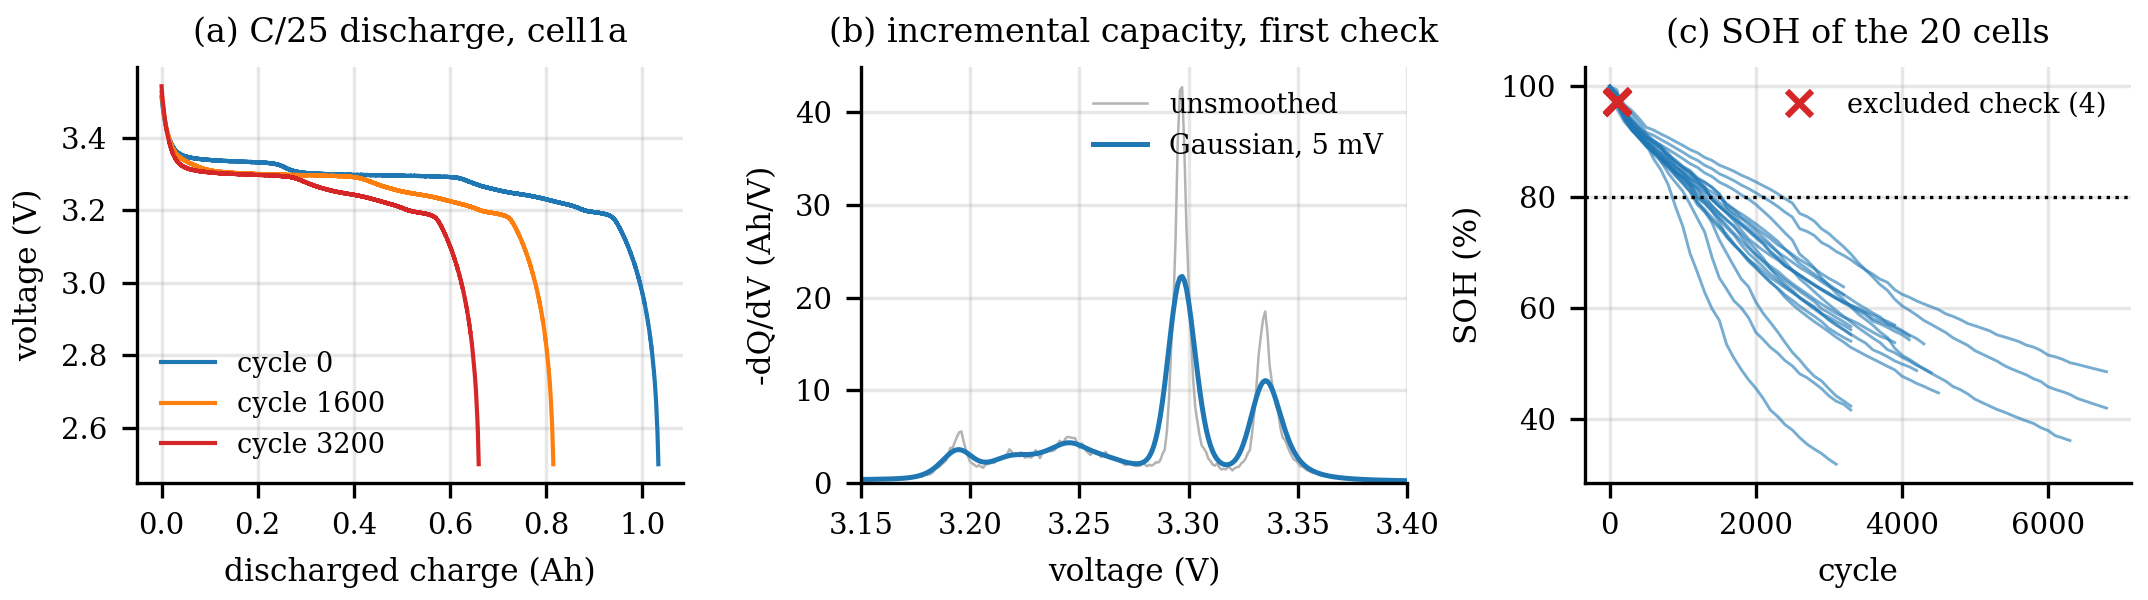
\includegraphics[width=\textwidth]{figures/preprocessing_s6.png}
  \caption{Preprocessing of S6. (a) C/25 discharge of one cell at three ages. (b) Incremental capacity at the first check, before and after Gaussian smoothing (5~mV), the source of the peak inputs. (c) SOH~\eqref{eq:soh} of the 20 cells over the 843 valid checks (crosses: the four excluded; dotted: 80\%).}
  \label{fig:prep}
\end{figure*}

\subsection{Big-data processing of the ageing cycles}
\label{sec:spark}

Between checks, every S6 cell logged each ageing cycle about once per second (827 files, 132~GB, $9.0\times10^{8}$ rows). Apache Spark~4.2 (PySpark, local mode) condenses them into the mean, last value and slope of seven measured quantities per 100-cycle block (21 inputs), each linked to the check that ends the block (details and validation in the supplement).

\subsection{State of health and forecasting target}
\label{sec:soh}
\label{sec:task}
\label{sec:features}

For cell $b$ with check capacities $C_{b,1}, C_{b,2},\dots$ in time order,
\begin{equation}
  \mathrm{SOH}_{b,k} = 100\,C_{b,k}/C_{b,1}\;\%,
  \label{eq:soh}
\end{equation}
the capacity-ratio definition~\cite{ref6,birkl2017}, here relative to the first valid measurement, not to the rated capacity. In S1 the capacity is the charge of the C/20 steps only~\cite[Eq.~(1)]{moy2024secondlife}; the processed tables also counted the pulse charge, shifting some labels by up to 0.09~pp.

A sample is a triple (cell $b$, origin $k$, horizon $h\in\{1,2,3\}$): a forecast made at check $k$ for check $k+h$, about one to three months ahead in S1 and 100--300 cycles in S6. The target is
\begin{equation}
  \Delta_{b,k,h} = \mathrm{SOH}_{b,k+h} - \mathrm{SOH}_{b,k},
  \label{eq:target}
\end{equation}
the multi-horizon target of~\cite{lim2021tft}, so an error in $\Delta$ is the same as the error in the future SOH. Errors are root-mean-square errors (RMSE) in SOH percentage points (pp). The fade rate $r_{b,k}$ is the ordinary least-squares slope~\cite{hastie2009elements} of SOH against time $t$ (days or cycles) over the last three valid checks,
\begin{equation}
  r_{b,k} = \frac{\sum_{i=k-2}^{k} (t_{b,i}-\bar t)(\mathrm{SOH}_{b,i}-\overline{\mathrm{SOH}})}{\sum_{i=k-2}^{k} (t_{b,i}-\bar t)^2}.
  \label{eq:fade}
\end{equation}

Inputs use only what is known at the origin. \textbf{F0} contains the SOH history ($\mathrm{SOH}_{b,k}$, time or cycles since the first check, $r_{b,k}$), fixed descriptors (S1: duty cycle and first-life history~\cite{moy2024secondlife}; S6: test conditions) and the \emph{planned} usage until the target (S1: days at each temperature set point and at rest; S6: cycles), so forecasts assume the planned usage is known. \textbf{F1} adds diagnostics measured at the origin: 47 in S1 (pulse resistances, incremental-capacity and EIS features) and 17 in S6 (plateau charges, incremental-capacity peaks, hysteresis, a resistance proxy). Test currents are excluded: in S1 they were set from the previous capacity and would give away the label. Missing values are filled from training data and flagged.

\subsection{Splits and protocols}
\label{sec:protocols}

\emph{Purged chronological splits.} Each cell's checks are cut at 60\% (A) and 80\% (B). Training targets lie at or before~A; validation samples start at or after~A and end by~B; test samples start at or after~B. Samples that straddle a cut are dropped, so no training label falls in the validation period and no validation label in the test period.

\emph{P1, continual stream.} A task is one cell in S1 (six tasks) or one test condition in S6 (seven tasks). At step $i$ of an ordering $\pi$, a method sees only the data of task $\pi_i$. Every method runs on the same 10 task orders with 5 seeds.

\emph{P2, unseen group.} One cell (S1) or condition (S6) is held out for testing, and models are trained on the rest.

\emph{P3, first-life pretraining.} All datasets are mapped onto shared inputs (SOH history, calendar and cycle time, planned time to the target, operating conditions and chemistry; undefined conditions flagged as missing). Models are first trained on the pool, which also sets the input scaling and the first EWC anchor; the seven S6 conditions then follow as a stream.

\subsection{Models}
\label{sec:backbones}

Preprocessing (standardisation, median imputation with missing indicators, target scaling) is fitted on the first task and then frozen. The \emph{MLP} has hidden layers of 128 and 64 ReLU units (dropout 0.1). The proposed model builds on the Temporal Fusion Transformer (TFT)~\cite{lim2021tft}: it looks at the $W{=}4$ most recent origins of the same cell and horizon (inputs only, never labels), which pass through per-variable embeddings, variable selection by gated residual networks, an LSTM encoder~\cite{hochreiter1997lstm} and two-head attention restricted to past steps (Fig.~\ref{fig:arch}; $d{=}8$, 12{,}708 parameters with the shared inputs).

% Proposed model, Residual TFT-EWC (Fig. 2). Drawn in TikZ; notation of Section III.
\begin{figure}[t]
  \centering
  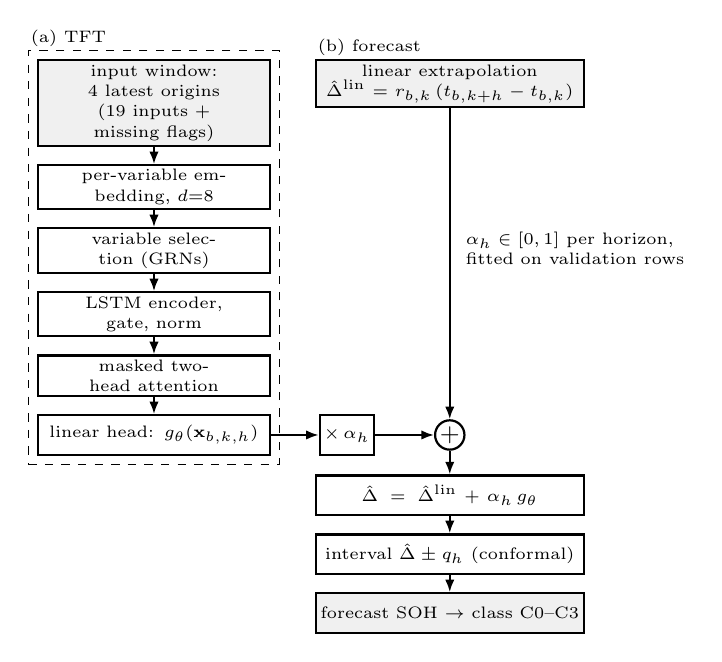
\begin{tikzpicture}[
      font=\fontsize{6.4}{7.4}\selectfont,
      blk/.style={draw, thick, rectangle, align=center, text width=2.85cm, minimum height=0.5cm, inner sep=1.5pt},
      side/.style={draw, thick, rectangle, align=center, text width=3.3cm, minimum height=0.5cm, inner sep=1.5pt},
      flow/.style={-{Latex[length=1.6mm]}, thick},
      node distance=0.22cm]
    % (a) correction network
    \node[blk, fill=black!6] (x) {input window: 4 latest origins\\ (19 inputs + missing flags)};
    \node[blk, below=of x] (emb) {per-variable embedding, $d{=}8$};
    \node[blk, below=of emb] (vsn) {variable selection (GRNs)};
    \node[blk, below=of vsn] (lstm) {LSTM encoder, gate, norm};
    \node[blk, below=of lstm] (att) {masked two-head attention};
    \node[blk, below=of att] (head) {linear head: $g_\theta(\mathbf{x}_{b,k,h})$};
    \foreach \a/\b in {x/emb, emb/vsn, vsn/lstm, lstm/att, att/head} \draw[flow] (\a) -- (\b);
    \node[draw, dashed, fit=(x)(head), inner sep=3pt] (tft) {};
    \node[anchor=south west, inner sep=1pt] at (tft.north west) {(a) TFT};

    % (b) forecast: head -> shrinkage -> sum <- linear extrapolation; sum -> forecast -> interval -> class
    \node[draw, thick, rectangle, minimum height=0.5cm, inner sep=1.5pt, right=0.6cm of head] (shr) {$\times\,\alpha_h$};
    \node[draw, thick, circle, inner sep=0.4pt, font=\small, right=0.75cm of shr] (sum) {$+$};
    \node[side, fill=black!6, anchor=north] (lin) at (sum |- x.north)
      {linear extrapolation\\ $\hat\Delta^{\mathrm{lin}}=r_{b,k}\,(t_{b,k+h}-t_{b,k})$};
    \node[anchor=south west, inner sep=1pt] at (lin.north west) {(b) forecast};
    \node[side, below=0.3cm of sum] (out) {$\hat\Delta=\hat\Delta^{\mathrm{lin}}+\alpha_h\,g_\theta$};
    \node[side, below=of out] (ci) {interval $\hat\Delta\pm q_h$ (conformal)};
    \node[side, fill=black!6, below=of ci] (cls) {forecast SOH $\rightarrow$ class C0--C3};
    \draw[flow] (head) -- (shr);
    \draw[flow] (shr) -- (sum);
    \draw[flow] (lin) -- (sum);
    \draw[flow] (sum) -- (out);
    \draw[flow] (out) -- (ci);
    \draw[flow] (ci) -- (cls);
    \node[align=left, anchor=west, font=\fontsize{6}{7}\selectfont] at ($(lin.south)!0.45!(sum.north)+(0.08,0)$)
      {$\alpha_h\in[0,1]$ per horizon,\\ fitted on validation rows};

  \end{tikzpicture}
  \caption{Proposed model, Residual TFT-EWC. (a) The TFT maps a window of the four latest origins of a cell to a
    correction $g_\theta$. (b) The correction is shrunk per horizon and added to linear
    extrapolation~\eqref{eq:residual}; conformal intervals give the reuse class. Each task is trained on
    the correction with the EWC penalty~\eqref{eq:ewc} (Fig.~\ref{fig:system}b).}
  \label{fig:arch}
\end{figure}


\emph{Strategies.} Fine-tuning trains on the current task only (a lower bound); experience replay~\cite{rolnick2019replay} keeps $B$ samples of each finished task; joint training fits all tasks at once (an upper bound); and Elastic Weight Consolidation (EWC)~\cite{kirkpatrick2017ewc} penalises changes to the weights that mattered for each finished task $j$,
\begin{equation}
  \frac{\lambda}{2}\sum_{p} F_{j,p}\,\big(\theta_p - \theta^{*}_{j,p}\big)^2,
  \label{eq:ewc}
\end{equation}
the penalty of~\cite[Eq.~(3)]{kirkpatrick2017ewc}, where $\theta^*_j$ are the parameters after task $j$ and $F_j$ is the empirical diagonal Fisher information over up to 500 training samples. \emph{TFT\,+\,EWC} is the proposed continual learner; trained on the residual~\eqref{eq:residual} below, with shrinkage and intervals, it becomes the proposed \emph{Residual TFT-EWC} (Fig.~\ref{fig:arch}). Training uses Adam~\cite{kingma2015adam}, batches of 64, at most 200 epochs and early stopping on the current task's validation RMSE.

\emph{Reference forecasters} are persistence ($\hat\Delta=0$), linear extrapolation of the fade rate, $\hat\Delta_{b,k,h} = r_{b,k}(t_{b,k+h}-t_{b,k})$, ridge regression (on planned usage only, F0 or F1) and histogram gradient boosting on F1.

\emph{Learned residual.} Because linear extrapolation proved hardest to beat, a follow-up experiment, registered in advance, trains the continual learners to correct it rather than replace it. With $\hat\Delta^{\mathrm{lin}}_{b,k,h}$ the extrapolation above (zero when $r_{b,k}$ is missing), the model $g_\theta$ learns $\Delta_{b,k,h}-\hat\Delta^{\mathrm{lin}}_{b,k,h}$ and the forecast is
\begin{equation}
  \hat\Delta_{b,k,h} = \hat\Delta^{\mathrm{lin}}_{b,k,h} + g_\theta(\mathbf{x}_{b,k,h}),
  \label{eq:residual}
\end{equation}
a residual hybrid of a simple and a learned forecaster, as in~\cite{zhang2003hybrid}.

\emph{Shrinkage and intervals.} After training, without changing the weights, the correction is scaled back per horizon by $\alpha_h=\min\!\big(1,\max(0,\sum p\,y/\sum p^2)\big)$, the least-squares slope through the origin~\cite{hastie2009elements} of the observed ($y$) on the predicted ($p$) correction on calibration rows. A split-conformal interval~\cite{lei2018conformal} $\hat\Delta\pm q_h$ takes as $q_h$ the $\lceil (n+1)(1-a)\rceil$-th smallest of the $n$ absolute calibration errors at horizon $h$. Intervals at level $1-a$ (90\% and 80\%) are scored by coverage, width and the interval score (Table~\ref{tab:metrics}; pp, lower is better). On the stream both are refitted after each task on its validation rows; extrapolation gets intervals the same way.

\emph{Registered experiments.} Each follow-up experiment was registered before it was run (Table~\ref{tab:exps}). Origins with a fade rate (H$^+$) and without one (H$^-$, a cell's first two checks, where extrapolation equals persistence) are reported separately. Horizons are 1--3 (E1) and 1--6 (E2); a question counts only if it replicates in both.

\begin{table}[t]
  \centering
  \caption{Registered follow-up experiments (all after P1--P3).}
  \label{tab:exps}
  \scriptsize
  \setlength{\tabcolsep}{2pt}
  \begin{tabular}{p{1.25cm}p{3.35cm}p{3.6cm}}
    \toprule
    Experiment & Setting & Question \\
    \midrule
    Residual & S6 stream, P3 inputs, from scratch & residual vs.\ direct target; beats extrapolation? \\
    SA-EWC & S6 stream & EWC penalty scaled by the input shift vs.\ fixed $\lambda$; BiLSTM~\cite{ref10}, TCN~\cite{ref8,ref10}, Transformer, GPR~\cite{ref3,ref4}, random forest, SVR (supplement) \\
    Shrinkage, intervals & S6 stream & shrunk residual model vs.\ extrapolation; interval coverage \\
    Unseen conditions & S6, P2; six training conditions streamed in the ten orders; shrinkage and intervals fitted once on pooled validation rows & beats extrapolation at H$^+$; vs.\ gradient boosting and joint TFT \\
    GB intervals & S6, P2; each training condition predicted by a model fitted on the other five (cross-validation interval~\cite{barber2021jackknife}, conditions as folds) & coverage on held-out conditions (no finite-sample guarantee) \\
    Many conditions & S7 (67 conditions), S10 (71); seven tune, the rest (60, 64) form five test folds & beats GB refitted on the stream's last condition, GB on all conditions, extrapolation (Wilcoxon over held-out conditions); S7 shrinks at every origin, S10 only at H$^+$ (rule fixed after S7) \\
    \bottomrule
  \end{tabular}
\end{table}

\subsection{Hyperparameters, metrics and statistics}
\label{sec:tuning}
\label{sec:metrics}

\emph{Tuning.} Hyperparameters are tuned on validation data from orders never used for evaluation, in two steps: first the learning rate of each backbone ($3\cdot10^{-4}$--$10^{-1}$), then the replay buffer $B$ (50--400) and the EWC strength $\lambda$ ($10^0$--$10^5$). A grid is extended if its best value lies on an edge. From P3 on, ten tuning orders are used, and the smallest value within one standard error of the best is kept.

\emph{Metrics.} After training step $i$, every task $j$ is tested, giving the error matrix $R_{i,j} = \mathrm{RMSE}(\mathcal{D}^{\mathrm{te}}_{\pi_j}\mid\theta_i)$~\cite{lopezpaz2017gem} over $T$ tasks. Table~\ref{tab:metrics} lists the metrics and their sources; positive BWT and forgetting mean forgetting. P2 adds standard error and class metrics, e.g.\ MAE, $R^2$, $R^2_\Delta$ of the change (${\le}0$ for persistence), MCC, Cohen's $\kappa_w$ and the AUC of SOH${\le}80\%$ (supplement Tables SI--SII).

\begin{table}[t]
  \caption{Evaluation metrics (BWT: backward transfer)}
  \label{tab:metrics}
  \centering
  \footnotesize
  \setlength{\tabcolsep}{3pt}
  \begin{tabular}{@{}lll@{}}
    \toprule
    Metric & Definition & Source \\
    \midrule
    Average error & $\tfrac{1}{T}\sum_{j} R_{T,j}$ & \cite{lopezpaz2017gem} \\
    BWT & $\tfrac{1}{T-1}\sum_{j<T} (R_{T,j} - R_{j,j})$ & \cite{lopezpaz2017gem} \\
    Forgetting & $\tfrac{1}{T-1}\sum_{j<T} \big(R_{T,j} - \min_{j\le i<T} R_{i,j}\big)$ & \cite{chaudhry2018rwalk} \\
    Skill & $1-\mathrm{RMSE}/\mathrm{RMSE}_{\mathrm{persist.}}$ & \cite{hyndman2006} \\
    Coverage & share of $\Delta$ inside $\hat\Delta\pm q_h$ & \cite{lei2018conformal} \\
    Interval score & $2q_h + \tfrac{2}{a}\max(|\Delta-\hat\Delta|-q_h,0)$ & \cite{gneiting2007scoring} \\
    Reuse class & C0 $>$95, C1 90--95, C2 80--90, C3 $\le$80\,\% & ours \\
    \bottomrule
  \end{tabular}
\end{table}

\emph{Statistics.} Means carry 95\% bootstrap intervals~\cite{efron1993bootstrap}. Methods are compared by two-sided Wilcoxon signed-rank tests~\cite{wilcoxon1945} on matched runs or held-out groups, with rank-biserial effect sizes~\cite{kerby2014rankbiserial} and Holm correction~\cite{holm1979}. A difference $d$ counts as \emph{replicated} only if, in both the main seed set (0--4) and a replicate set (5--9), it is significant, has the same sign and $|d|\ge 0.05$~pp. If $|d|<0.05$~pp in both, the methods are practically equivalent. This threshold is about half the label shift caused by the pulse-charge definition.

\subsection{Implementation and availability}
\label{sec:repro}

The pipeline uses Python~3.11, NumPy~2.4, pandas~3.0, scikit-learn~1.9 and PyTorch~2.14.1 (P1 and P2 were first run on an Intel Xeon with an unrecorded PyTorch version and re-run on an Intel Core~5~210H), with one CPU thread and seeded, deterministic algorithms. Every result file records configuration, seeds, library versions and the Git commit, and unit tests cover input causality, split purging and label exclusion. The datasets are at doi:10.17605/OSF.IO/8JNR5 (S1), 10.57745/OLBXKT (S6), 10.35097/1969 (S7), 10.5281/zenodo.10963339 (S8), 10.5281/zenodo.6405084 (S9) and 10.6084/m9.figshare.25975315 (S10). Code, decision log, pre-registrations and results: \url{https://github.com/TarunSitaraman/continual-learning-heterogeneous-second-life-ev-batteries}.


% =============================================================================
% Results (condensed to the IEEE conference length)
%
% Numbers are from committed results files produced on clean commits:
% results/forecasting.json (S1, d710cad), results/forecasting_wheeler.json (S6,
% 53ab76f), their re-runs (docs/RESULTS.md, Reproducibility check),
% results/forecasting_d21_p3.json (57e37aa), results/forecasting_d21_ablation_a1*.json
% and results/d21_tft_interpretation.json; D23 and D24 from
% results/forecasting_d23_e*.json (5ae2f84) and results/forecasting_d24_e*.json (947b33a); D25-D27 from
% results/forecasting_d25_e*.json (a59debb), results/forecasting_d26_e*.json (9866d7a) and
% results/forecasting_d27_e*.json (494b36f), D28 and D29 from results/forecasting_d28_e*.json (161c01f) and
% results/forecasting_d29_e*.json (f2fdd73), D32 from results/forecasting_d32_e*.json (fdcf0d6),
% summarised in docs/RESULTS.md. Table headline is generated by scripts/make_headline_table.py; table d26
% (now in the supplement) is written from those files by hand. Other tables are generated by
% scripts/make_results_tables.py; figures by
% scripts/make_d25_d27_figures.py and scripts/make_d28_figures.py.
% =============================================================================

\section{Results}
\label{sec:results}

% Generated by scripts/make_headline_table.py from results/forecasting_d23/d25/d26/d32/d35_e*.json
\begin{table*}[t]
  \centering
  \caption{The proposed model against the two strongest traditional forecasters on S6, in both settings. Top:
    test RMSE (pp); proposed model: mean over 50 runs, main/replicate seed sets; others: single deterministic fits
    (bold: best). Bottom: proposed minus baseline (pp, main/replicate; negative favours the proposed model) and the
    verdict of the replication rule (better/worse: significant after Holm in both seed sets, same sign, at least
    0.05~pp; equiv.: below 0.05~pp in both; n.r.: not replicated). $^\ast$Post hoc for the shrunk model; registered
    for the unshrunk model (D23), with the same verdict. $^\dagger$Under the continual constraint of the proposed
    model (conditions one at a time, earlier data not kept): refitted on the newest condition (P2: D32; P1: D35,
    residual target, the more accurate of its two forms). $^\ddagger$Post hoc (D35).}
  \label{tab:headline}
  \setlength{\tabcolsep}{4pt}
  \footnotesize
  \begin{tabular}{lcccc}
    \toprule
    & \multicolumn{2}{c}{Continual stream (P1)} & \multicolumn{2}{c}{Unseen usage condition (P2)} \\
    \cmidrule(lr){2-3}\cmidrule(lr){4-5}
    & $h{=}1$--3 & $h{=}1$--6 & $h{=}1$--3 & $h{=}1$--6 \\
    \midrule
    \textbf{Residual TFT-EWC} (proposed) & \textbf{0.32/0.31} & 0.50/0.49 & 0.92/0.94 & 1.62/1.65 \\
    Linear extrapolation & 0.34 & \textbf{0.48} & 1.37 & 2.30 \\
    Gradient boosting, all conditions stored & 0.45 & 0.90 & \textbf{0.54} & \textbf{1.05} \\
    Gradient boosting, latest condition only$^\dagger$ & 0.56 & 0.96 & 0.86 & 1.59 \\
    Persistence & 1.64 & 2.67 & 2.82 & 4.90 \\
    \midrule
    \multicolumn{5}{l}{\emph{Proposed minus baseline, verdict}} \\
    vs.\ linear extrapolation & $-0.02$/$-0.04$ equiv. & $+0.01$/$+0.01$ equiv. & $-0.45$/$-0.43$ better & $-0.68$/$-0.65$ better \\
    vs.\ gradient boosting, all stored & $-0.13$/$-0.14$ better$^\ast$ & $-0.40$/$-0.41$ better$^\ast$ & $+0.39$/$+0.41$ worse & $+0.57$/$+0.60$ worse \\
    vs.\ gradient boosting, latest only$^\dagger$ & $-0.24$/$-0.25$ better$^\ddagger$ & $-0.46$/$-0.46$ better$^\ddagger$ & $+0.06$/$+0.08$ worse & $+0.03$/$+0.06$ n.r. \\
    \bottomrule
  \end{tabular}
\end{table*}


\emph{Summary.} Neither traditional forecaster is reliable in both settings (Table~\ref{tab:headline}; pairs such as 0.32/0.31 give the main and replicate seed sets). Gradient boosting, which sees every condition's data at once, is best on an unseen condition, yet 0.13--0.41~pp less accurate than the proposed model on the continual stream (replicated; post hoc for the shrunk model). Linear extrapolation is the mirror image: level with the proposed model on the stream, 0.43--0.68~pp less accurate on an unseen condition (replicated). The proposed model is level with or better than each where the other fails. Held to the same constraint (one condition at a time, no earlier data kept), gradient boosting refitted on the latest condition is slightly more accurate for horizons 1--3 (0.06/0.08~pp, replicated) and not distinguishable for 1--6; warm-started boosting cannot use the usage inputs after the first condition and is far worse (supplement).

\emph{Data.} S1 diagnostics track the current SOH (median within-cell $\rho=0.97$ for the main incremental-capacity peak) but not the change to the next RPT (median $|\rho|\le0.3$); every S1 sample stays in class C0, while all S6 cells cross from C0 to C3.

% -----------------------------------------------------------------------------
\subsection{Continual stream (P1)}
\label{sec:res-p1}

\emph{S1.} The methods are practically equivalent: TFT\,+\,EWC reaches 0.462~pp (skill 0.27), level with gradient boosting, TFT fine-tuning and MLP replay (0.466--0.475~pp; Table~SIV of the supplement), ridge on the planned usage alone reaches 0.450~pp, and forgetting is small throughout (0.016--0.040~pp).

\emph{S6.} When tasks differ in usage, forgetting is substantial (0.18--0.46~pp). EWC lowers the TFT's error relative to fine-tuning (0.677 against 0.883~pp), though which difference is significant changed between runs (\S\ref{sec:res-repro}); the MLP beats the TFT in both runs (0.531--0.540~pp), joint training puts the TFT's continual-learning cost at about 0.25~pp, and linear extrapolation (0.343~pp) and gradient boosting (0.372~pp) are best.

% -----------------------------------------------------------------------------
\subsection{Unseen cell or usage condition (P2)}
\label{sec:res-p2}

% Generated by scripts/make_results_tables.py from results/forecasting.json (commit d710cad), results/forecasting_wheeler.json (commit 53ab76f)
\begin{table}[t]
  \centering
  \caption{Protocol P2 (unseen battery in S1, unseen usage condition in S6): mean test RMSE (pp) over held-out groups, range over groups. Reuse-class metrics of the same forecasts: Table~\ref{tab:d30_cls_s6}.}
  \label{tab:p2}
  \setlength{\tabcolsep}{3pt}
  \begin{tabular}{llcc}
    \toprule
    Data & Method & RMSE & Range \\
    \midrule
    S1 & Persistence & 0.545 & 0.436--0.688 \\
    S1 & Linear extrapolation & 0.511 & 0.284--0.725 \\
    S1 & Ridge, usage only & 0.301 & 0.172--0.409 \\
    S1 & Ridge, F0 & 0.418 & 0.158--0.779 \\
    S1 & Ridge, F1 & 0.320 & 0.161--0.477 \\
    S1 & Gradient boosting, F1 & 0.219 & 0.091--0.299 \\
    S1 & MLP & 0.285 & 0.149--0.389 \\
    S1 & TFT & 0.292 & 0.199--0.377 \\
    \midrule
    S6 & Persistence & 2.817 & 2.025--4.327 \\
    S6 & Linear extrapolation & 1.372 & 0.856--1.669 \\
    S6 & Ridge, usage only & 1.177 & 0.870--2.288 \\
    S6 & Ridge, F0 & 0.859 & 0.598--1.836 \\
    S6 & Ridge, F1 & 1.137 & 0.588--2.188 \\
    S6 & Gradient boosting, F1 & 0.710 & 0.395--1.839 \\
    S6 & MLP & 0.821 & 0.476--2.225 \\
    S6 & TFT & 0.868 & 0.551--2.390 \\
    \bottomrule
  \end{tabular}
\end{table}


Gradient boosting is best on both datasets (Table~\ref{tab:p2}). On S6 the 100\% depth-of-discharge condition is the hardest for every method (1.8--2.4~pp). With six or seven held-out groups, no difference with the TFT survives Holm correction.

In the further metrics, gradient boosting has the largest $R^2_\Delta$ (0.54 on S1, 0.74 on S6), while extrapolation forecasts the change no better than its mean ($-1.31$, $-0.05$). The S6 reuse class gives the same order (Table~\ref{tab:d30_cls_s6}; MCC 0.93 for gradient boosting, 0.72 for persistence).

% Generated by scripts/make_d30_outputs.py from results/forecasting_d30_s6.json (commit cb43efb)
\begin{table}[t]
  \centering
  \caption{S6, P2: reuse class (C0--C3) and end of first life (EoL, SOH $\le$ 80) of the forecast SOH, held-out samples pooled, mean over seeds; F1 macro, $\kappa_w$ linear-weighted. All metrics and class counts: Table~SII of the supplement.}
  \label{tab:d30_cls_s6}
  \setlength{\tabcolsep}{3pt}
  \scriptsize
  \begin{tabular}{lcccccc}
    \toprule
    Method & Acc. & F1 & MCC & $\kappa_w$ & EoL F1 & EoL AUC \\
    \midrule
    Persistence & 0.858 & 0.661 & 0.723 & 0.809 & 0.962 & 0.998 \\
    Linear extrapolation & 0.939 & 0.777 & 0.876 & 0.909 & 0.989 & 0.999 \\
    Ridge, usage only & 0.954 & 0.851 & 0.905 & 0.932 & 0.989 & 0.999 \\
    Ridge, F0 & 0.963 & 0.881 & 0.922 & 0.942 & 0.990 & 0.999 \\
    Ridge, F1 & 0.958 & 0.852 & 0.912 & 0.935 & 0.986 & 0.999 \\
    Gradient boosting, F1 & 0.966 & 0.893 & 0.928 & 0.948 & 0.989 & 0.999 \\
    MLP & 0.962 & 0.871 & 0.921 & 0.942 & 0.989 & 0.999 \\
    TFT & 0.963 & 0.882 & 0.923 & 0.943 & 0.989 & 0.999 \\
    \bottomrule
  \end{tabular}
\end{table}


\emph{Reproducibility.}\label{sec:res-repro} A re-run of P1 and P2 in a pinned environment, on data rebuilt from the raw archives, reproduced every baseline, every P2 result and the ranking of methods. The neural models moved by at most 0.059~pp, enough to change the significance of differences of 0.005--0.014~pp: neural training is deterministic per platform, not across platforms. This motivated the stricter tuning and the replication rule used from P3 on.

% -----------------------------------------------------------------------------
\subsection{First-life pretraining (P3)}
\label{sec:res-p3}

Pretraining on the first-life pool (36{,}711 samples, against 2{,}409 in S6) does not help. Both backbones are better from scratch on average (TFT 0.401/0.415~pp against 0.509/0.591~pp pretrained with EWC, significant only in the replicate set), and linear extrapolation (0.343~pp) remains the most accurate method, on S6 and on the pool's own test split (supplement).

\emph{Why the TFT improved.} A post hoc ablation, repeated on the replicate seeds, explains why the TFT from scratch improves from 0.891 to 0.401~pp with the shared inputs: dropping the 17 diagnostic features (0.17--0.35~pp) and adding the calendar time between checks (0.19--0.31~pp), both replicated ($p_{\mathrm{Holm}}\le0.002$).
\label{sec:res-interp}

% -----------------------------------------------------------------------------
\subsection{Learned residual on linear extrapolation}
\label{sec:res-residual}

\begin{figure*}[t]
  \centering
  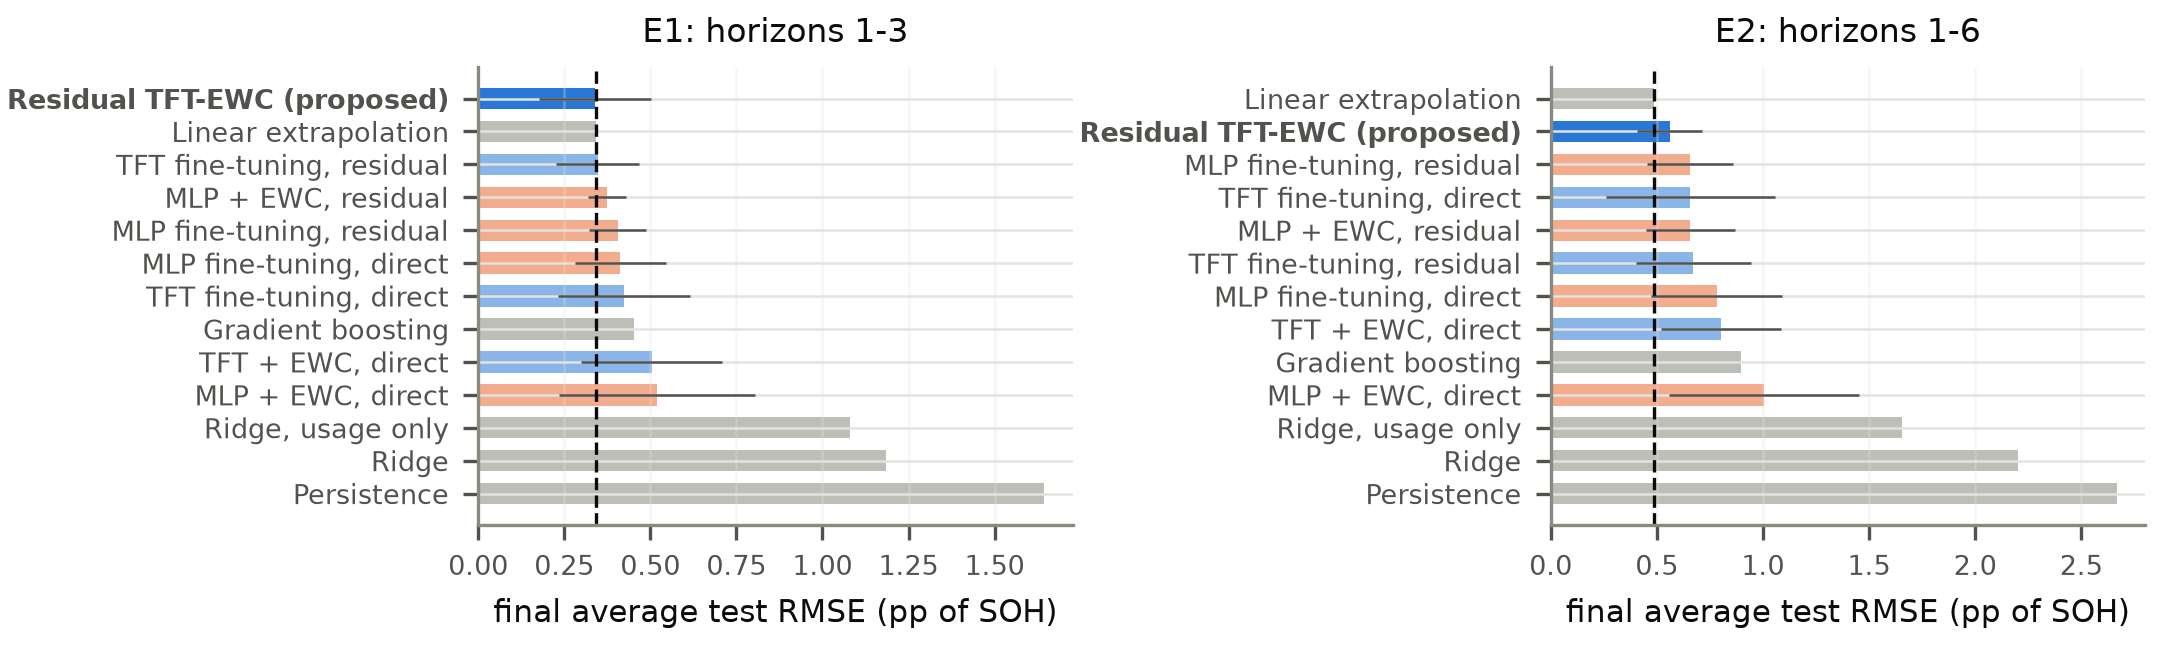
\includegraphics[width=\textwidth]{figures/d23_comparison.png}
  \caption{S6 continual stream: final average test RMSE (pp), mean and s.d.\ over the 50 runs of the main seed
    set; bold, blue: the proposed residual TFT-EWC; dashed: linear extrapolation. Replicate set, forgetting and
    literature backbones: Table~SIII of the supplement.}
  \label{fig:d23bar}
\end{figure*}

Learning the residual~\eqref{eq:residual} (Fig.~\ref{fig:d23bar}; Table~SIII of the supplement) did \emph{not} meet the pre-registered criterion of beating linear extrapolation: the two are practically equivalent for horizons 1--3, and for 1--6 extrapolation is slightly better on average (not replicated); per horizon it is better at $h=1$--2 (replicated), and the gap closes by $h=5$--6. It does make the TFT competitive: 0.17~pp (E1) and 0.24--0.30~pp (E2) more accurate than the direct form and ahead of gradient boosting, all replicated. For horizons 1--6, where it forgets more, EWC lowers its forgetting from 0.28/0.22 to 0.09~pp and its backward transfer from 0.18/0.14 to 0.03~pp, replicated; its effect on the final error is not. For horizons 1--3, EWC and fine-tuning are practically equivalent. \emph{Ageing-cycle inputs.} The 21 Spark-extracted inputs (Section~\ref{sec:spark}), added as pre-specified, make the residual TFT\,+\,EWC worse: 0.480/0.501 against 0.339/0.314~pp, and worse than linear extrapolation, both replicated.

% -----------------------------------------------------------------------------
\subsection{Shift-adaptive EWC and literature baselines}
\label{sec:res-d24}

The second pre-registered criterion, for SA-EWC (Table~SIII of the supplement), was \emph{not} met: although the shift weights varied (0.05--1.14), SA-EWC and fixed $\lambda$ are practically equivalent in final error and forgetting (differences of at most 0.03~pp). For horizons 1--3, BiLSTM\,+\,EWC (direct, 0.323~pp, and residual) and the residual Transformer\,+\,EWC are practically equivalent to the residual TFT; for 1--6 it beats the residual BiLSTM and TCN (replicated; not the Transformer). Every single-fit regressor is worse than the residual TFT\,+\,SA-EWC (replicated), except the residual SVR for horizons 1--6.

% -----------------------------------------------------------------------------
\subsection{Shrinkage and intervals on the stream}
\label{sec:res-d25}

Shrinking the correction per horizon makes the residual TFT\,+\,EWC practically equivalent to extrapolation at every horizon (0.318/0.308 against 0.343~pp for horizons 1--3, 0.498/0.493 against 0.485~pp for 1--6), removing its loss at $h=1$--2, but the criterion was again not met. Its 90\% intervals are narrower than extrapolation's but cover too little (0.71--0.81, against 0.92--0.95), so the interval scores are equal. Pretraining the residual model on the first-life pool makes it worse for horizons 1--3 (by 0.22~pp, replicated) and does not help for 1--6.

% -----------------------------------------------------------------------------
\subsection{Residual model on unseen conditions}
\label{sec:res-d26}

On unseen conditions (Table~\ref{tab:headline}; Table~SV of the supplement), the shrunk residual TFT\,+\,EWC beats extrapolation, as registered, at origins with a fade rate (by 0.12~pp for horizons 1--3 and 0.18--0.20~pp for 1--6, replicated), its first win over extrapolation. At a cell's first two checks, extrapolation reduces to persistence and loses by over 2~pp. Gradient boosting, however, is 0.39--0.41~pp (horizons 1--3) and 0.57--0.60~pp (1--6) more accurate than the TFT (replicated), on six of the seven conditions; only on the 100\% depth-of-discharge condition is the TFT better. The same residual TFT trained jointly improves on its continual form by 0.32--0.44~pp (replicated), and shrinkage makes no practical difference.

\begin{figure}[t]
  \centering
  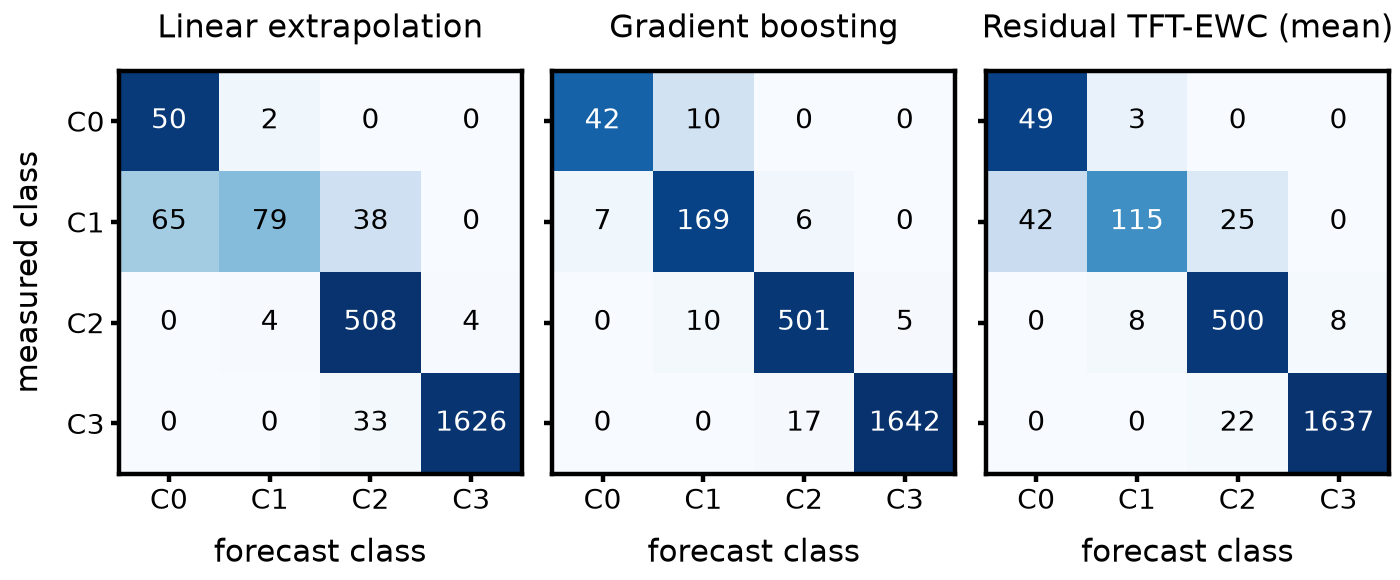
\includegraphics[width=\columnwidth]{figures/d26_confusion.png}
  \caption{Reuse-class confusion on unseen S6 conditions (Table~SVI of the supplement): sample counts (proposed model: mean over 50 runs); shading: share of the measured class.}
  \label{fig:d26cm}
\end{figure}

The capacity-based classes follow the same ranking (Table~SVI of the supplement, Fig.~\ref{fig:d26cm}): the proposed model assigns the measured class to 95.5\% of held-out samples (94.4--96.8\% over the 50 runs), against 93.9\% for extrapolation and 85.8\% for persistence, while ridge (96.5\%) and gradient boosting (97.7\%) do better. All errors are between neighbouring classes; the most common is the risky one for reuse, a measured C1 sample forecast as C0 (65 of 182 for extrapolation, 42 for the proposed model, 7 for gradient boosting).

\emph{Intervals on unseen conditions.} Intervals calibrated on validation rows of the training conditions cover too little on the held-out one (0.66--0.68 for the TFT and 0.74--0.76 for extrapolation, at 90\%). The calibration rows are much of the cause: calibrating extrapolation, which has no fitted parameters, on every origin of those conditions raises its coverage to 0.89--0.90. Gradient-boosting intervals calibrated by leaving one condition out reach the registered 0.85 (0.90) with the lowest interval scores (3.2 and 6.7~pp), though their advantage over calibrated extrapolation is significant only for horizons 1--3 (not established). Pooled coverage hides one failure: the 100\% depth-of-discharge condition, outside the others' range, is covered only 0.48 and 0.38 (Fig.~S8, supplement).

\emph{Refit and tracking.} As the held-out condition's checks arrive, refitting gradient boosting and tracking the half-width lower its mean 90\% interval score by 29\%, from 3.22 to 2.29~pp ($h{=}1$--3; six of seven conditions, $p=0.047$) and from 6.67 to 4.74~pp ($h{=}1$--6; seven of seven, $p=0.016$), with pooled coverage 0.90--0.91. On the 100\% depth-of-discharge condition coverage rises from 0.48/0.38 to 0.72/0.58, short of the registered 0.80. Then 87--93\% of held-out intervals lie within one reuse class, 99.2--99.7\% of them correctly.

% ============================================================
% V. DISCUSSION and VI. CONCLUSION (condensed to the IEEE conference length)
% Every number is taken from docs/RESULTS.md and the committed results files.
% ============================================================

\section{Discussion}
\label{sec:discussion}

\emph{Where the proposed model is strongest.} Extrapolation trails on new conditions and gradient boosting on the stream; Residual TFT-EWC holds up in both. Matching extrapolation is itself hard: fade is smooth and tasks are small (21--27 and 135--225 training samples in S1 and S6). Most of the gap to gradient boosting and joint training on unseen conditions comes from storing earlier data, not from the model (Section~\ref{sec:res-many}). Where earlier data cannot be kept (privacy, ownership, volume), continual learning is the natural choice; here, storing every group was still cheap.

\emph{What drives its accuracy.} Building on the best simple forecaster mattered most. The ablation points to the inputs, not the architecture: the calendar time between checks helps because at 50~$^\circ$C all 20 S6 cells lose more capacity per cycle when checks are further apart.

\emph{Reuse.} The reuse classes screen on relative capacity alone, while reuse also depends on power, safety, absolute capacity and cost. For a group unlike any seen before, such as the 100\% depth-of-discharge condition, neither forecasts nor intervals can be trusted, and pooled coverage hides this.

\emph{Limitations.} We switched to forecasting after inspecting the first dataset, and decided the ablation and all later experiments after the main results (all but the ablation registered before being run; the stream test of gradient boosting refitted on the newest condition is post hoc; S7 and S10 were added to find a setting where the model wins, the S10 rule after the S7 results). The second-life datasets are small; S6 is aged at 50~$^\circ$C and its ``second life'' continues the same test; SOH is relative to each cell's first valid measurement; forecasts assume the planned usage is known. The TFT settings for unseen conditions were tuned on validation rows of all seven S6 conditions, from one laboratory, and leave-one-condition-out intervals cover only gradient boosting and extrapolation.

\section{Conclusion}
\label{sec:conclusion}

We proposed Residual TFT-EWC, a continual learner that forecasts second-life SOH as a scaled-down correction to linear extrapolation. It is the only model compared that holds up both on the stream (level with extrapolation, ahead of gradient boosting, far less forgetting with EWC) and on unseen conditions (ahead of extrapolation, and of gradient boosting held to the same rule on all 64 unseen S10 conditions). Gradient boosting and joint training, which keep all earlier data, stay more accurate there. Intervals held only when calibrated on conditions left out of training, and not outside the training range. Future work should test settings where data cannot be stored and groups are larger, and add power and safety criteria to the screening.

% ============================================================
% REFERENCES
% ============================================================

\bibliographystyle{IEEEtran}
\bibliography{references}

\end{document}
